\chapter{Definition Logging, Tracing {\fontfamily{bch}\selectfont \&} Monitoring}\label{ch:definition-von-logging-tracing-&-monitoring}
Es existiert kein fehlerfreies IT-System.
%TODO: besser formulieren, ltm unterstützen den prozess ein fehlerhaftes system zu verbessern und zu perfektionieren.
Daher muss ein Prozess zu einem funktionierenden System geschaffen werden.
Logging zeichnet auf, was eine Anwendung macht.
Tracing protokolliert, wenn eine Anwendung andere Service aufruft.
%TODO: Aufrufe von services
Monitoring zieht aus diesen Informationen Schlüsse, um Fehler einer Anwendung aufzudecken.
Wenn die gefundenen Fehler ausgebessert werden, kommt man dem fehlerfreien System näher.
Im Folgenden werden die drei Verfahren genauer erklärt.


\section{Logging}\label{sec:logging}
Als Logging wird das automatische Protokollieren von Ereignissen bezeichnet.
Hierzu zählen Fehlermeldungen, Systemnachrichten, Statusmeldungen, etc.
Die Daten, die protokolliert werden, werden in eine oder mehrere Log-Dateien geschrieben.
Diese Dateien enthalten die Ereignisse mit Zeitstempel, welche meist chronologisch geschrieben werden.
\\
Außerdem werden die einzelnen Logs mit einem Loglevel versehen, womit der Entwickler das Protokoll besser auswerten kann.
Es gibt sechs verschiedene Loglevel.
Das schwerwiegendste Level heißt \enquote{Fatal}, hierbei spiegeln die Logs wider, dass die Applikation in einem katastrophalen Zustand ist und eingegriffen werden muss.
Falls dieses Level auftritt, sollte sofort eingegriffen werden, um die Applikation wieder verfügbar zu machen.
Das zweite Loglevel nennt sich \enquote{Error}, hierbei läuft die Applikation weiter, ist aber auf einen Fehler getroffen.
Der Administrator sollte die Anwendung so früh wie möglich untersuchen und den Fehler beheben.
Das nächste Level für Logs ist \enquote{Warning}.
Die Applikation ist in einem Zustand, der nicht üblich ist.
Dieser sollte analysiert werden, um wieder in den Normalzustand zu gelangen.
Da die Anwendung läuft, hat die Fehlerbehebung nicht die höchste Priorität, sollte trotzdem zeitnah erledigt werden.
Als viertes Loglevel wird \enquote{Information} bezeichnet.
Dieses Level wird in der produktiven Umgebung genutzt, um Interessantes im Produktionssystem nachvollziehen zu können.
In Testumgebungen wird das Loglevel \enquote{Debug} genutzt, um weitere Informationen auswerten zu können.
Das letzte Loglevel wird \enquote{Verbose} genannt, hierbei werden alle Details einer Anwendung dokumentiert.
Durch das gesetzte Loglevel können die Logs in einem Protokoll nach diesem Parameter gefiltert werden.
Hierfür muss eine einheitliche Struktur der Logs gewährleistet sein.
\\
\\
Das Log-Management kümmert sich um die langfristige Speicherung, sodass die Daten über lange Zeit nachvollziehbar sind.
Hierbei sollten die Logs an einer zentralen Stelle gespeichert werden, wie zum Beispiel einer Datenbank.
Logs sollten bestimmten Standards entsprechen, um die Integration mit zentralisierten Protokollierungsdiensten zu erleichtern.
Die Logs können kurzfristig auch in der Konsole ausgegeben werden, können dadurch aber nicht langzeitig ausgewertet.
Lokale Speicherung der Logs in Dateien erschweren das Auswerten.
%TODO Visualisierung
\\
Das Event-Management stellt Funktionen bereit, um diese Daten auswerten zu können.
Zusammengefasst Log- und Event-Management sammeln die Log-Daten, speichern sie, sodass die Daten genutzt werden können, um Probleme zu identifizieren, Prozesse nachzuvollziehen, Systemleistung zu optimieren oder Cyberangriffe und andere Sicherheitsvorfälle zu erkennen und abzuwehren.
\\
\\
Logs helfen dabei Sicherheitsvorfälle zu identifizieren.
Falls gegen Richtlinien verstoßen wird, fallen diese in den Logs durch die Überwachung auf.
In den Protokollen werden Informationen festgehalten, um Probleme und ungewöhnliches Verhalten nachvollziehen zu können.
\\
Manche Logs sind durch den Gesetzgeber verpflichtend, um Ereignisse nachverfolgen zu können.
Transaktionen im Bankumfeld sind verpflichtend aufzuzeichnen, um die Nachvollziehbarkeit dieser Aktionen sicherzustellen.
Im Gesundheitswesen ist Logging gesetzlich gefordert, um Compliance-Richtlinien zu erfüllen.
Unter anderem gilt die Datenschutzgrundverordnung, um die Daten richtig zu verarbeiten.
\\
\\
Durch künstliche Intelligenz oder maschinelles Lernen können große Datenmengen automatisiert organisiert und ausgewertet werden.
Logging sollte innerhalb einer Anwendung einheitlich verwendet werden.
Das Logging sollte in der gesamten Organisation konsistent verwendet werden, um die Ereignisse, die in den Protokollen abgelegt sind, mit Ereignissen verschiedener Systeme vergleichen und verwalten zu können.
\\
Die geloggten Ereignisse können aus verschiedenen Quellen protokolliert sein.
Falls es eine Client-Software ist, können die Aktionen auf dem Desktop oder mobilen Gerät aufgezeichnet werden.
Bei der Nutzung einer Datenbank sollten diese Aufrufe protokolliert werden.
Beim Auslesen, Verändern oder Löschen eines Datensatzes sollten diese als Ereignisse im Protokoll aufgenommen werden.
Falls vertrauliche Daten abgelegt sind, müssen diese auch vertraulich in den Logdateien abgelegt sein.
Der Vertraulichkeitsgrad muss beibehalten werden, um die Daten weiterhin zu schützen.
\\
Um die Sicherheitsstandards, die Alarmierung und Berichterstattung zu erfüllen, müssen das Niveau und der Inhalt in der Anforderungsanalyse und Entwurfsphase entwickelt und festgehalten werden.
Niveau und Inhalt sollte in einem angemessenen Verhältnis zu dem Informationsrisiko stehen.
Hierfür gibt es keine einheitliche Checkliste, da jedes Unternehmen, Organisation und Anwendung verschieden sind.
\\
\\
Jeder Eintrag in einem Protokoll muss \enquote{wann, wo, wer und was} aufzeichnen.
Wann steht hierbei für den Zeitstempel des Ereignisses mit Datum und Uhrzeit in einem internationalen Format.
Dieser kann vom Protokollierungszeitpunkt abweichen.
Wo steht für die Kennung der Anwendung, beispielsweise der Name und die Version.
Die Anwendungsadresse sollte auch protokolliert sein, hierzu zählt die IP-Adresse und Portnummer des Servers.
Wer ist aufgeteilt in menschlicher und maschineller Benutzer.
Zum einen die Quelladresse, beispielsweise die IP-Adresse des Benutzers oder die Mobiltelefonnummer.
Zum anderen die Benutzeridentität, falls dieser authentifiziert ist, zum Beispiel der Benutzername oder die Lizenznummer.
Was steht für die Schwere des Ereignisses, also dem Loglevel, und die Beschreibung des Ereignisses.
Weitere mögliche Aufzeichnungen sind HTTP-Statuscodes oder interne Einordnung.
\\
Manche Ereignisse dürfen nicht direkt in die Protokolle geschrieben werden.
Sie müssen gesondert behandelt werden, entweder entfernt, maskiert, gehasht oder verschlüsselt werden.
Daten wie Quellcode, sensible Informationen oder Authentifizierungskennwörter gehören zu diesen besonders zu behandelnden Ereignissen.
Verschlüsselungsschlüssel und andere Geheimnisse müssen geschützt werden.
Inhaberdaten von Bankkonten und Zahlungskarten müssen besonders geschützt gespeichert werden.
Anders zu behandeln sind Daten wie Dateipfad, interne Netzwerkdaten oder nicht sensible personenbezogene Daten.
Hierfür muss die Organisation selbst entscheiden, wie sensibel diese Daten protokolliert werden sollen.
\\
\\
Nach Möglichkeit sollten Fehler bei der Eingabevalidierung in den Logs gespeichert werden.
Authentifizierungserfolge und -fehler sollten protokolliert werden.
Zugriff sollte kontrolliert werden und Autorisierungsfehler sollten geloggt werden.
Anwendungsfehler und Systemereignisse, beispielsweise wie Laufzeitfehler oder Verbindungsprobleme, sollten im Protokoll gespeichert werden.
Um Anwendungen und verwandte Systeme zu überwachen, sollte jeder Start und Stop aufgezeichnet werden.
Optional sollten weitere Ereignisse protokolliert werden, um die Sicherheit einer Anwendung zu erhöhen.
Übermäßiger Gebrauch sollte dokumentiert sein.
In den Protokollen sollte verdächtiges oder unerwartetes Verhalten einer Anwendung oder eines Systems erkennbar sein.
\\
\\
Die Protokolle mit den gesammelten Ereignissen müssen nach dem Speichern vor Missbrauch geschützt werden.
Beispielsweise müssen Daten vor unbefugten Zugriff bewahrt werden.
Manche Protokolle enthalten Daten, die der Konkurrenz dienen können.
Geschäftliche Werte können Journalisten von Nutzen sein, um Schätzungen über Einnahmen zu machen.\autocite{ip-insider, ait, owasp}


\section{Tracing}\label{sec:tracing}
Ein Trace ist die direkte Visualisierung eines Requests beim Durchlauf durch eine Anwendung oder eine komplette Anwendungslandschaft.
Tracing macht es möglich, nachzuvollziehen, in welchen Zuständen ein Objekt zuvor war.
Allerdings erhöht Tracing die Komplexität des Codes und ist daher besser geeignet für Microservicearchitekturen.
Ein Trace zeichnet die verschiedenen Aufrufe auf, beispielsweise einen HTTP-Request oder einen Datenbankaufruf.
Während der Entwicklung einer Anwendung können Zusatzinformationen zum Verarbeitungsprozess nützlich sein.
Neben den üblichen Ausgaben einer Anwendung helfen die Zusatzinformationen beim Testen der Anwendung.
\\
\\
Bei Microservices hilft das Distributed Tracing und es bezeichnet die verteilte Rückverfolgung.
Hierbei werden einzelne Prozesse getrennt und somit wird erkennbar, wo Probleme entstanden sind.
Um bei Problemen den verursachenden Microservice zu identifizieren, erhält jeder Prozess eine Profil-ID.
Jeder Microservice signiert jede Nutzungsanfrage mit dieser ID.
Alle Prozesse lassen sich so einem bestimmten Service zuordnen, identifizieren und analysieren.
Falls nun ein Fehler auftritt, lässt sich der Microservice, der den fehlerhaften Prozess ausführt, durch die ID identifizieren.
Insgesamt ist die Fehlersuche vereinfacht.
Des Weiteren unterstützt Tracing beim Debugging.
\\
Tracing wird in verschiedenen Arten spezifiziert.
Im allgemeinen Gebrauch für Anwendungen wird als Trace der Aufruf anderer Systeme bezeichnet.
Während der Pandemie haben wir das ortsbezogene Tracing kennengelernt.
Hierbei ist ein Trace die Nachverfolgung eines bestimmten Ereignisses, beispielsweise der Besuch einer Gastronomie.
Außerdem gibt es das nähebezogene Tracing.
Hierfür werden die Personen bzw. deren Geräte nachverfolgt und geschätzt wer, wie nah und wie lange in der Nähe war.
\\
\\
Oft wird Tracing mit Tracking verglichen oder sogar verwechselt.
Der Unterschied liegt dabei, dass Tracking den aktuellen Zustand beschreibt, wie zum Beispiel die GPS-Koordinaten einer Bestellung.
Tracing beschreibt das Nachverfolgen, für das gleiche Beispiel wird beim Tracing der Bestelleingang, Verarbeitungsprozess etc. protokolliert.\autocite{adesso, monstarlab, dev-insider}


\section{Monitoring}\label{sec:monitoring}
Monitoring sammelt viele Daten und zielt darauf ab, richtige Schlüsse zu ziehen.
Ein einfaches Beispiel, das Monitoring sollte erkennen, dass ein Problem vorliegt, wenn eine Komponente ausfällt.
Hierfür wird die Anwendung konstant überwacht und der Status aller Komponenten erfasst.
Des Weiteren werden die Daten der Anwendung oder Systems aufbereitet und bewertet, sodass sie in einer übersichtlichen Zusammenfassung präsentiert werden können.
Durch Monitoring fallen Abweichungen vom Normalzustand auf, dadurch sollte ein Alarm ausgelöst werden, um den Nutzer aufzufordern den Fehler zu beheben.
Je nach Schweregrad des Fehlers werden verschiedene Medien zum Benachrichtigen des Nutzers verwendet.
Bei schweren Fehlern kann eine SMS auf das Arbeitstelefon geschickt werden.
Bei leichteren Fehlern kann eine Email reichen.
\\
\\
\begin{figure}[h]
    \centering
    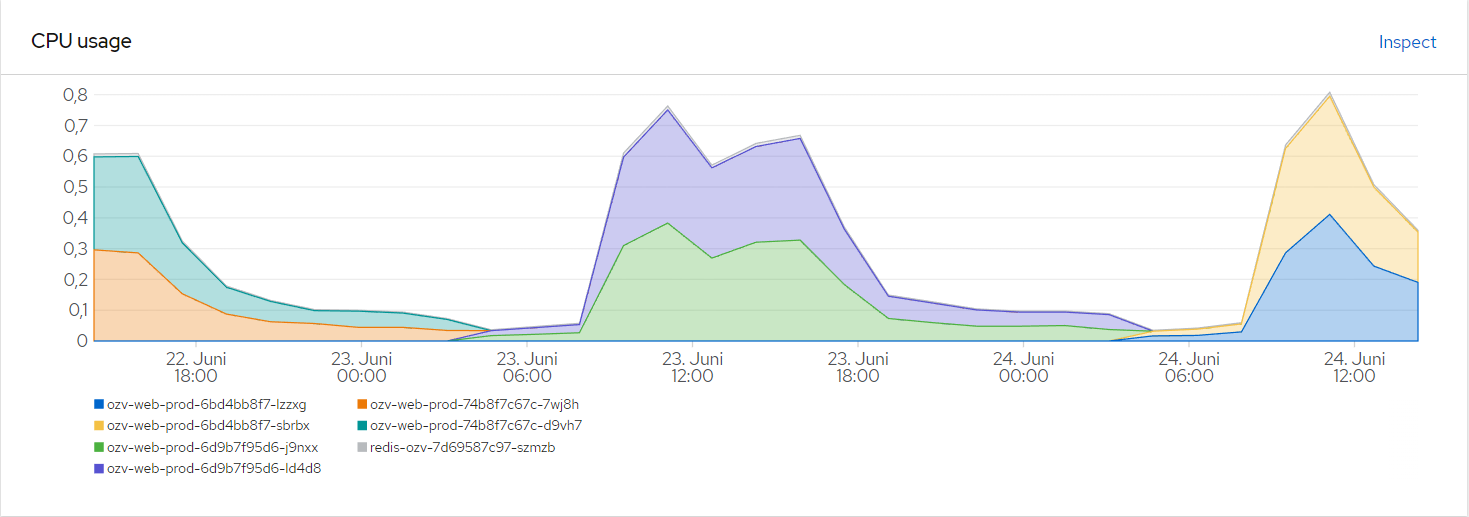
\includegraphics[width=\linewidth]{images/cpu-ozv-web}
    \caption{CPU-Auslastung über 2 Tage}\label{fig:figure}
\end{figure}
\\
Durch den Vergleich zu historischen Daten soll das Monitoring-System Aussagen über die Zuverlässigkeit einer Anwendung treffen.
Durch das Überwachen einer Anwendung können Ausfälle vermieden und vorgebeugt werden.
Ein Interface des Monitorings zeigt die Performance und Auslastung der Komponenten, die durchgehend gemessen werden.
Diese Überwachung wird genutzt, um Hardwareausstattung zu planen.
\\
\\
Anforderungen an ein Monitoring-System können in fünf Kategorien unterteilt werden.
Zunächst beobachtet das Monitoring den \enquote{Zustand des Systems}.
Hierzu gehört das \enquote{End-to-End}-Monitoring, welches die ausgelieferten Daten so nah wie möglich am Endnutzer auf Funktionalität überprüft.
Zur Zustandserfassung gehört die Statuserfassung der Dienste, unter anderem die Hardwareauslastung, als auch die Softwareüberwachung.
Des Weiteren werden diese Informationen für lange Zeit gespeichert, um die Verfügbarkeit von Diensten und Komponenten zu analysieren.
Die zweite Kategorie ist die \enquote{Alarmierung}, welche das manuelle Eingreifen verlangt.
Hierbei wird ein Mitarbeiter über die Ursache des Fehlers informiert.
Die Reaktionszeit und Fehlerbehebung wird dokumentiert.
Die nächste Kategorie wird als \enquote{Diagnose} bezeichnet, hierbei werden Informationen gesammelt, um die Ursachenanalyse von Fehlern detailliert zu ermöglichen.
Die gesammelten Informationen dienen der Entscheidungsfindung.
Die vierte Kategorie ist die \enquote{Qualitätsmessung}.
Es werden Daten gesammelt, die über die Leistungsfähigkeit und den Durchschlag von Systemen und Anwendungen Aufschluss geben.
Außerdem werden vereinbarte Grenzwerte und deren Einhaltung erfasst.
Dadurch können Engpässe und Überlastungen aufgedeckt werden.
Die letzte Kategorie ist die \enquote{Konfiguration}.
Hierfür werden standardisierte Konfigurationen überwacht und bei Abweichungen von standardisierten Vorgehen gewarnt.
\\
\\
Monitoring bietet viele Vorteile.
Unter Anderem werden die Abhängigkeiten zwischen Anwendungen abgebildet.
Außerdem werden Trendanalysen genutzt, um den Einsatz von Rechenleistung und Ressourcen zu verbessern.
\\
Monitoring ist in zwei Arten vorhanden.
Einmal gibt es das \enquote{Historical Monitoring}, welches proaktives Arbeiten fordert.
Hierbei muss der Admin vorausschauend das Handeln planen.
Mit Langzeitstatistiken werden Kapazitäten geplant und können die Budgetplanung des Unternehmens unterstützen.
Der Admin erkennt die Missstände, informiert die Betroffenen und entwirft Lösungsansätze.
Die zweite Art des Monitoring ist das \enquote{Real-Time-Monitoring}.
Hierbei werden die Server überwacht und bei Problemen direkt reagiert.
Im Idealfall werden Fehler registriert und behoben, bevor der Nutzer diesen bemerkt.\autocite{cloudradar, wbs, crossmedia}

%\section{Sinnvolle Nutzung}\label{sec:sinnvolle-nutzung}
%\section{Sinnvolle Ausgaben}\label{sec:sinnvolle-ausgaben}
%\section{Wann ist es übertrieben?}\label{sec:wann-ist-es-übertrieben?}
